\chapter{Hopf algebras}
In this chapter we give the definition of $k$-algebras, $k$-coalgebra, $k$-bialgebras and Hopf algebras. For this we fix an arbitrary field $k$. We start by reintroducing the notion of a $k$-algebra in terms of diagrams, where we require all $k$-algebras to be unitary and associative. Then we dualize this concept to obtain the notion of a $k$-coalgebra. Combining the previous two we arrive at $k$-bilalgebras, which will then lead to definition of a Hopf algebra by equipping a $k$-bialgebra with an antipodel map.

Most of the definitions and diagrams in this chapter are taken from \cite{Brown}.





\section{algebras, coalgebra and bialgebras}



\subsection{\texorpdfstring{$k$}{k}-algebras}


\begin{defi}
 For any $k$-vector space let
 \[
  \tau_A \colon A \otimes A \to A \otimes A, \quad a \otimes b \mapsto b \otimes a
 \]
 be the \emph{flip map} (of $A$).
\end{defi}


\begin{defi}\label{defi: algebras via diagrams}
 A $k$-algebra is a tupel $(A, m, u)$ consisting of a $k$-vector space $A$, linear maps $m \colon A \otimes A \to A$, called the \emph{multiplication} and a linear map $u \colon k \to A$, called the \emph{unit} such that the following two diagrams commute, where $s$ denotes the respective scalar multiplication.
 \begin{center}
  \tikzsetnextfilename{associativity_of_algebras}
  \begin{tikzpicture}[node distance = 5em]
   \node (AAA) {$A \otimes A \otimes A$};
   \node[right = 5em of AAA] (AA1) {$A \otimes A$};
   \node[below of = AAA] (AA2) {$A \otimes A$};
   \node[below of = AA1] (A) {$A$};
   \draw[->] (AAA) to node[above] {$m \otimes \id_A$} (AA1);
   \draw[->] (AAA) to node[left] {$\id_A \otimes\, m$} (AA2);
   \draw[->] (AA1) to node[right] {$m$} (A);
   \draw[->] (AA2) to node[below] {$m$} (A);
  \end{tikzpicture}
  \quad
  \tikzsetnextfilename{unit_of_algebras}
  \begin{tikzpicture}[node distance = 3em]
   \node (middle) {$ $};
   \node[above of = middle] (AA) {$A \otimes A$};
   \node[left = 5em of middle] (kA) {$k \otimes A$};
   \node[right = 5em of middle] (Ak) {$A \otimes k$};
   \node[below of = middle] (A) {$A$};
   \draw[->] (kA) to node[above left] {$u \otimes \id_A$} (AA);
   \draw[->] (Ak) to node[above right] {$\id_A \otimes \, u$} (AA);
   \draw[->] (AA) to node[right] {$m$} (A);
   \draw[->] (kA) to node[below left]  {$s$} (A);
   \draw[->] (Ak) to node[below right] {$s$} (A);
  \end{tikzpicture}
 \end{center}
 The commutativity of the left diagram is the \emph{associativity aximion} and the commutativity of the right diagram is the \emph{unit axiom}. The $k$-algebra $(A, m, u)$ is called \emph{commutative} if the following diagram commutes:
 \begin{center}
  \tikzsetnextfilename{commutativity_of_algebras}
  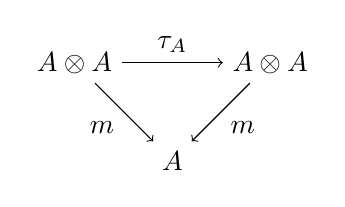
\begin{tikzpicture}[node distance = 5em]
   \node (AA1) {$A \otimes A$};
   \node[below right of = AA1] (A) {$A$};
   \node[above right of = A] (AA2) {$A \otimes A$};
   \draw[->] (AA1) to node[above] {$\tau_A$} (AA2);
   \draw[->] (AA1) to node[below left] {$m$} (A);
   \draw[->] (AA2) to node[below right] {$m$} (A);
  \end{tikzpicture}
 \end{center}
\end{defi}


\begin{rem}
 Definition \ref{defi: algebras via diagrams} is equivalent to the usual definition of a $k$-algebra, namely a $k$-vector space $A$ together with a bilinear map $\hat{m} \colon A \times A \to A, (a,b) \mapsto a \cdot b$ which is associative in the sense that $(a \cdot b) \cdot c = a \cdot (b \cdot c)$ for all $a,b,c \in A$, and such that a unit $1 \in A$ exists, i.e.\ an element for which $1 \cdot a = a \cdot 1 = a$ for every $a \in A$.
 
 Given a $k$-algebra in the usual sense the multiplication $\hat{m}$ corresponds to a linear map $m \colon A \otimes A \to A, a \otimes b \mapsto a \cdot b$, and that $m$ satisfies the associativity axiom is equivalent to $\hat{m}$ being associative. That a linear map $u \colon k \to A$ satisfies the unit axiom is equivalent to $u(1)$ being a unit in $A$. That $(A,\hat{m})$ is commutative is then also equivalent to $(A,m,u)$ being commutative.
\end{rem}


\begin{expl}
 Let $G$ be any group. Then the \emph{group algebra} $k[G]$ is defined by the underlying vector space being $kG$, the free vector space with basis $G$, and the multiplication which arises from extending the multiplication of $G$ linearly, i.e.
 \[
  \left( \sum_{g \in G} \lambda_g g \right) \cdot \left( \sum_{h \in G} \mu_h h \right)
  = \sum_{g,h \in G} (\lambda_g \mu_h) (gh)
  = \sum_{g \in G} \left( \sum_{h \in G} \lambda_{gh^{-1}} \mu_h \right) g.
 \]
 The associativity of the multiplication can be checked by direct calculation. The unit of the group algebra $k[G]$ is given by the identity of the group $e \in G \subseteq k[G]$. The group algebra $k[G]$ is commutative if and only if $G$ is.
\end{expl}


\begin{defi}
 Let $A$ and $B$ be $k$-algebras. A linear map $f \colon A \to B$ is a \emph{homomorphism of $k$-algebras} if the following two diagrams commute:
 \begin{center}
  \raisebox{-\height}{
  \tikzsetnextfilename{homomorphism_of_algebras_multiplication}
  \begin{tikzpicture}[node distance = 5em]
   \node (AA) {$A \otimes A$};
   \node[right = 5em of AA] (BB) {$B \otimes B$};
   \node[below of = AA] (A) {$A$};
   \node[below of = BB] (B) {$B$};
   \draw[->] (AA) to node[above] {$f \otimes f$} (BB);
   \draw[->] (A) to node[below] {$f$} (B);
   \draw[->] (AA) to node[left] {$m_A$} (A);
   \draw[->] (BB) to node[right] {$m_B$} (B);
  \end{tikzpicture}}
  \hspace{0.5cm}
  \raisebox{-\height}{
  \tikzsetnextfilename{homomorphism_of_algebras_unit}
  \begin{tikzpicture}[node distance = 5em]
   \node (A) {$A$};
   \node[below right = of A] (k) {$k$};
   \node[above right = of k] (B) {$B$};
   \draw[->] (A) to node[above] {$f$} (B);
   \draw[->] (k) to node[below left] {$u_A$} (A);
   \draw[->] (k) to node[below right] {$u_B$} (B);
  \end{tikzpicture}}
 \end{center}
\end{defi}




\subsection{\texorpdfstring{$k$}{k}-coalgebras}


\begin{defi}
 A $k$-coalgebra is a tupel $(C,\Delta,\varepsilon)$ consisting of a $k$-vector space $C$, a linear map $\Delta \colon C \to C \otimes C$, called the \emph{comultiplication} and a linear map $\varepsilon \colon C \to k$, called the \emph{counit}, such that the following two diagrams commute:
 \begin{center}
  \tikzsetnextfilename{coassociativity_of_coalgebras}
  \begin{tikzpicture}[node distance = 5em]
   \node (C) {$C$};
   \node[right = 7em of C] (CC1) {$C \otimes C$};
   \node[below of = C] (C2) {$C \otimes C$};
   \node[below of = CC1] (CCC) {$C \otimes C \otimes C$};
   \draw[->] (C) to node[above] {$\Delta$} (CC1);
   \draw[->] (C) to node[left] {$\Delta$} (CC2);
   \draw[->] (CC1) to node[right] {$\id_C \otimes\, \Delta$} (CCC);
   \draw[->] (CC2) to node[below] {$\Delta \otimes \id_C$} (CCC);
  \end{tikzpicture}
  \quad
  \tikzsetnextfilename{counit_of_coalgebras}
  \begin{tikzpicture}[node distance = 3em]
   \node (middle) {$ $};
   \node[above of = middle] (CC) {$C \otimes C$};
   \node[left = 5em of middle] (kC) {$k \otimes C$};
   \node[right = 5em of middle] (Ck) {$C \otimes k$};
   \node[below of = middle] (C) {$C$};
   \draw[->] (CC) to node[above left] {$\varepsilon \otimes \id_C$} (kC);
   \draw[->] (CC) to node[above right] {$\id_C \otimes \, \varepsilon$} (Ck);
   \draw[->] (C) to node[right] {$\Delta$} (CC);
   \draw[->] (C) to node[below left]  {$1 \otimes \id_C$} (kC);
   \draw[->] (C) to node[below right] {$\id_C \otimes\, 1$} (Ck);
  \end{tikzpicture}
 \end{center}
 The commutativity of the left diagram is the \emph{coassociativity axiom} and the commutativity of the right diagram is the \emph{counit axiom}. The coalgebra $(C, \Delta, \varepsilon)$ is called \emph{cocommutative} if the following diagram commutes:
 \begin{center}
  \tikzsetnextfilename{cocommutativity_of_coalgebras}
  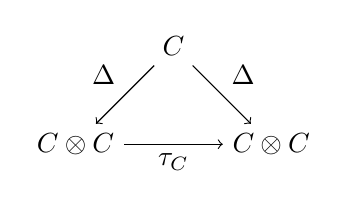
\begin{tikzpicture}[node distance = 5em]
   \node (CC1) {$C \otimes C$};
   \node[above right of = CC1] (C) {$C$};
   \node[below right of = C] (CC2) {$C \otimes C$};
   \draw[->] (CC1) to node[below] {$\tau_C$} (CC2);
   \draw[->] (C) to node[above left] {$\Delta$} (CC1);
   \draw[->] (C) to node[above right] {$\Delta$} (CC2);
  \end{tikzpicture}
 \end{center}
\end{defi}


\begin{expls}
 \begin{enumerate}[leftmargin=*]
  \item
   Let $C$ be a $k$-vector space and $(x_i)_{i \in I}$ a basis of $V$. Then $V$ carries the structure of a $k$-coalgebra via the comultiplication $\Delta \colon C \to C \otimes C$ defined by
   \[
    \Delta(x_i) \coloneqq x_i \otimes x_i \quad \text{for every $i \in I$}
   \]
   and the counit $\varepsilon \colon C \to k$ defined by
   \[
    \varepsilon\left( \sum_{i \in I} \lambda_i x_i \right) \coloneqq \sum_{i \in I} \lambda_i.
   \]
   To see that $\Delta$ is coassociative notice that for every $i \in I$
   \begin{align*}
     ((\id_C \otimes\, \Delta) \circ \Delta)(x_i)
     &= (\id_C \otimes\, \Delta)(x_i \otimes x_i)
     = x_i \otimes x_i \otimes x_i \\
     &= (\Delta \otimes \id_C)(x_i \otimes x_i)
     = ((\Delta \otimes \id_C) \circ \Delta)(x_i).
   \end{align*}
   To notice that $\varepsilon$ is a counit notice that for every $i \in I$
   \[
     ((\varepsilon \otimes \id_C) \circ \Delta)(x_i)
     = (\varepsilon \otimes \id_C)(x_i \otimes x_i)
     = 1 \otimes x_i
     = (1 \otimes \id_C)(x_i)
   \]
   and similarly $(\id_C \otimes\, \varepsilon) \circ \Delta = \id_C \otimes\, 1$.
   
  \item
   At a special case of the above example it follows that for any group $G$ the group algebra $k[G]$ also carries the structure of a $k$-coalgebra via the comultiplication $\Delta \colon k[G] \to k[G] \otimes k[G], g \mapsto g \otimes g$ and counit $\varepsilon \colon k[G] \to k, \sum_{g \in G} \lambda_g g \mapsto \sum_{g \in G} \lambda_g$.
 \end{enumerate}
\end{expls}

